\documentclass[a4paper,11pt,fleqn]{scrartcl}
\usepackage{../../Styles/Cours}

\newcommand{\chnum}{Chapitre 8}
\newcommand{\chtitle}{De la structure à la polarité d'une entité}
\newcommand{\dtype}{cours}

\pgfdeclarelayer{background}
\pgfsetlayers{background,main}

\usetikzlibrary{calc}

% --------- Liaison simple (inchangée) ----------
\newcommand{\Bond}[6]%
% start, end, thickness, incolor, outcolor, iterations
{ \begin{pgfonlayer}{background}
    \colorlet{InColor}{#4}
    \colorlet{OutColor}{#5}
    \foreach \I in {#6,...,1}
    {   \pgfmathsetlengthmacro{\r}{#3/#6*\I}
        \pgfmathsetmacro{\C}{sqrt(1-\r*\r/#3/#3)*100}
        \draw[InColor!\C!OutColor, line width=\r]
        (#1.center) -- (#2.center);
    }
  \end{pgfonlayer}
}
\newcommand{\SingleBond}[2]%
{   \Bond{#1}{#2}{1mm}{white}{gray!50}{10} }
% --------- Liaison double ----------
\newcommand{\DoubleBond}[2]%
% start, end
{
    % distance de séparation
    \def\Offset{0.8mm}

    % vecteur normal unitaire
    \path let
        \p1 = (#1.center),
        \p2 = (#2.center),
        \n1 = {veclen(\x2-\x1,\y2-\y1)}
    in
    coordinate (N) at ({-(\y2-\y1)/\n1},{(\x2-\x1)/\n1});

    % deux liaisons décalées
    \Bond{#1}{#2}{0.8mm}{white}{gray!50}{10}
    \begin{pgfonlayer}{background}
        \foreach \s in {-1,1}
        {
            \draw[line width=0.8mm, gray!60]
            ($(#1.center)+\s*\Offset*(N)$) --
            ($(#2.center)+\s*\Offset*(N)$);
        }
    \end{pgfonlayer}
}

% --------- Liaison triple ----------
\newcommand{\TripleBond}[2]%
% start, end
{
    \def\Offset{1mm}

    \path let
        \p1 = (#1.center),
        \p2 = (#2.center),
        \n1 = {veclen(\x2-\x1,\y2-\y1)}
    in
    coordinate (N) at ({-(\y2-\y1)/\n1},{(\x2-\x1)/\n1});

    % liaison centrale
    \Bond{#1}{#2}{0.7mm}{white}{gray!50}{10}

    % deux liaisons latérales
    \begin{pgfonlayer}{background}
        \foreach \s in {-1,1}
        {
            \draw[line width=0.7mm, gray!60]
            ($(#1.center)+\s*\Offset*(N)$) --
            ($(#2.center)+\s*\Offset*(N)$);
        }
    \end{pgfonlayer}
}



\begin{document}
    \maketitle
\section{Etablir un schéma de Lewis}
    \subsection{Les règles du duet et de l'octet}
    Dans une molécule, chaque atome respecte la règle du duet ou la règle de l'octet. Les formuules de Lewis des molécules permettent de vérifier le respect de ces règles en comptabilisant les électrons des liaisons covalentes et des doublets non-liants pour chaque atome de la molécule.
    \subsection{Etablie un schéma de Lewis}
    La méthode suivante permet d'établir en 4 étapes le schéma de Lewis d'une molécule :
    \begin{cours}
    \begin{itemize*}
        \item Ecrire la configuration électronique de chaque atome
        \item Déterminer le nombre total d'électrons de valence $n_t$ mis en jeu dans la molécule étidiée.
        \item Déterminer le nombre de doublets d'électrons (impliqués dans des liaisons ou des doublets non liants) en divisant le nombre $n_t$ par deux.
        \item Répartir les doublets en respectant les règles du duet (pour H) et de l'octet pour les autres atomes. Chaque atome forme un nombre de liaisons covalentes égal au nombre d'électrons manquant pour respecter la règle de l'octet ou du duet.
    \end{itemize*}
    \end{cours}

    \begin{exemple}
    Pour la molécule d'amoniac \ce{NH3}
    \begin{center}
        \begin{tabular}{|m{.2\linewidth}|m{.15\linewidth}|m{.15\linewidth}|m{.15\linewidth}|m{.15\linewidth}|}
            \hline
            \textbf{Molécule} & \multicolumn{4}{c|}{\ce{NH3}}\\
            \hline
            \textbf{Atomes} & H & H & H & N\\
            \hline
            \textbf{Configuration électronique}& & & & \\
            \hline
            \textbf{Electrons de valence} & & & & \\
            \hline
            \textbf{Electrons manquants pour respecter la règle} & & & & \\
            \hline
            $n_t$ &  \multicolumn{4}{c|}{}\\
            \hline
            \textbf{Nombre de doublets} &  \multicolumn{4}{c|}{}\\
            \hline
            \textbf{Répartition et nature des doublets} &  \multicolumn{4}{c|}{}\\
            \hline
        \end{tabular}
    \end{center}
    \end{exemple}
    \subsection{Pour aller plus loin : les acides de Lewis}
    Les atomes porteurs d'une lacune électronique ne respectent pas la règle de l'octet ou du duet et sont donc susceptibles de créer une liaison covalente avec un doublet non-liant d'une autre molécule.
    \begin{exemple}
        La molécule de borane \ce{BH3} :\\
        \vspace{4em}
    \end{exemple}

\section{La géométrie spatiale des molécules}
    \subsection{Géométrie d'une molécule}
    On peut prévoir la géométrie d'une entité chimique à partir de sa structure de Lewis. Autour d'un atome qualifié de "central", les doublets liants, ou doublets des liaisons covalentes, et les doublets non-liants s'écartent au maximum les uns des autres afin de minimiser les forces de répulsion électrostatique.\\
    Les réométries adoptées sont des formes géométriques simples :
    \begin{center}
        \begin{tabular}{|m{.2\linewidth}|m{.2\linewidth}|m{.2\linewidth}|m{.2\linewidth}|}
            \hline
            \textbf{Nombre de liaison (simples ou doubles) et de doublets liants}  & \textbf{Géométrie autour de l'atome central} & \textbf{Répartition spatiale} & \textbf{Exemple}\\
            \hline
            2 liaisons & Linéaire & \rule{0pt}{3em} & \\
            \hline
            2 liaisons simples et une liaison double & Plane trigonale  & \rule{0pt}{4em}& \\
            \hline
            4 liaisons simples & Tétraédrique & \rule{0pt}{4em}& \\
            \hline
            5 liaisons simples & Bipyramide trogonale & \rule{0pt}{5em}& \\
            \hline
            6 liaisons simples & Octaèdre & \rule{0pt}{5em} & \\
            \hline
        \end{tabular}
    \end{center}
    \begin{exemple}
        A partir de la représentation de Lewis de la molécule d'ammoniac (\ce{NH3}), indiquer la géométrie adoptée.\\
        \vspace{5em}
    \end{exemple}

\section{Polarité des molécules}
    \subsection{Electronégativité et polarisation}
    L'électronégativité d'un atome, notée par la lettre grecque $\chi$ (khi) traduit son aptitude à attirer à lui les électrons d'une liaison dans laquelle il est engagé. Cette grandeur sans unité varie en fonction de la place de l'élément chimique dans le tableau périodique.\\
    Dans une liaison covalente entre deux atomes $A$ et $B$, si l'atome $A$ est plus électronégatif que l'atome $B$, la liaison $A-B$ est dite polarisée. On calculera alors $\Delta \chi$, la différence d'électronégativité  : $$\Delta \chi = \chi(A) - \chi(B) $$
    Si $\Delta \chi >0.5$ alors la liaison sera considérée comme polarisée. Elle est alors notée $A^{\delta +} - B^{\delta -}$.\\
    Les symboles $\delta +$ et $\delta -$ traduisent les charges partielles portées par les atomes de cette liaison covalente : $A$ étnt plus électronégatif, il porte une charge partielle négative notée $\delta -$, et $B$ porte une charge partielle notée  $\delta +$.

    \subsection{Prévoir la polarité d'une molécule}
    Une molécule peut être polaire si elle comporte au moins une liaison polarisée :
    \begin{itemize}
        \item si elle ne comporte qu'une liaison polarisée, elle est alors nécessairement polaire
        \item si elle comporte plusieurs liaisons polarisées, il faut alors étudier la géométrie de cette molécule pour s'assurer que la polarisation des liaisons ne se compense pas.
    \end{itemize}
    \begin{exemple}
        Polarité des molécules d'eau et de dioxyde de carbone :\\
        \vspace{10em}
    \end{exemple}
\end{document}

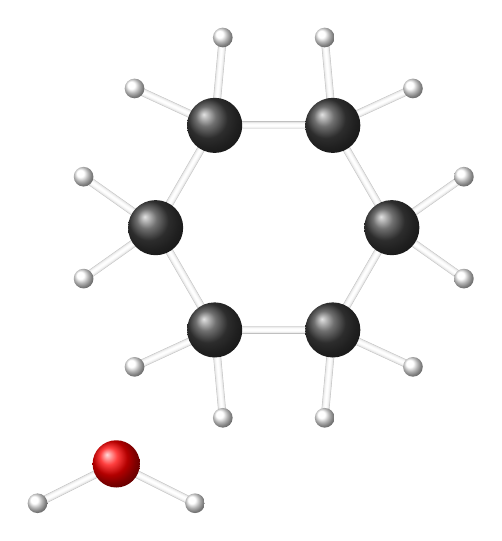
\begin{tikzpicture}
[   oxygen/.style={circle, ball color=red, minimum size=6mm, inner sep=0},
    hydrogen/.style={circle, ball color=white, minimum size=2.5mm, inner sep=0},
    carbon/.style={circle, ball color=black!75, minimum size=7mm, inner sep=0}
]
    \node[oxygen] (O1) at (0,0) {};
    \node[hydrogen] (H1) at (1,-0.5) {};
    \node[hydrogen] (H2) at (-1,-0.5) {};
    \SingleBond{O1}{H1}
    \SingleBond{O1}{H2}

    \foreach \c in {1,...,6}
    {   \node[carbon] (C-\c) at ($(2,3)+(\c*60:1.5)$) {};
        \node[hydrogen] (H-\c-a) at ($(2,3)+(\c*60-15:2.5)$) {};
        \node[hydrogen] (H-\c-b) at ($(2,3)+(\c*60+15:2.5)$) {};
        \SingleBond{C-\c}{H-\c-a}
        \SingleBond{C-\c}{H-\c-b}
    }
    \foreach \c [evaluate={\c as \n using int(mod(\c,6)+1)}] in {1,...,6}
    {   \SingleBond{C-\c}{C-\n}
    }
\end{tikzpicture}

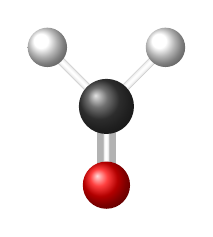
\begin{tikzpicture}
[   oxygen/.style={circle, ball color=red, minimum size=6mm, inner sep=0},
    hydrogen/.style={circle, ball color=white, minimum size=5mm, inner sep=0},
    carbon/.style={circle, ball color=black!75, minimum size=7mm, inner sep=0}
]
    \node[carbon] (C1) at (0,0) {};
    \node[hydrogen] (H1) at (-.75,.75) {};
    \node[hydrogen] (H2) at (.75,.75) {};
    \node[oxygen] (O) at (0,-1) {};
    \SingleBond{C1}{H1}
    \SingleBond{C1}{H2}
    \DoubleBond{C1}{O}
\end{tikzpicture}